%
% tensor.tex -- Tensoralgebra (Indexgymnastik)
%
% (c) 2017 Prof Dr Andreas Müller, Hochschule Rapperswil
%
\chapter{Tensoren}
\lhead{Tensoren}
\rhead{}
Matrizen und Vektoren sind ein- und zweidimensionale Anordnungen von
Zahlen.
Matrizen operieren linear auf Vektoren und erzeugen neue Vektoren.
Kann dieses Konzept verallgemeinert werden auf Operationen, die
auf mehreren Vektoren oder sogar Matrizen wirken?
Tensoren beantworten diese Frage.

%
% motivation.tex -- Motivation der Tensoralgebra
%
% (c) 2017 Prof Dr Andreas Müller, Hochschule Rapperswil
%
\section{Multilineare Algebra%
\label{section:multilinearealgebra}}
\rhead{Multilineare Algebra}
In der elementaren linearen Algebra begnügt man sich damit, lineare
Abbildungen zu studieren.
Der Matrizenkalkül stellt sich in diesem Zusammenhang als eine
besonders erfolgreiche und intuitive Notation heraus.
Doch bereits beim Skalarprodukt stösst die Notation an ihre Grenzen,
die bei multilinearen Funktionen von mehr als zwei Vektoren
endgültig überschritten werden.
Dieses Kapitel sucht daher nach einem erweiterten Kalkül, der mit
diesen allgemeineren Situationen fertig werden kann.

\subsection{Multilineare Funktionen%
\label{subsection:multilinearefunktionen}}
Die multiplikative Grundoperation der Matrizenalgebra ist die 
Multiplikation $\text{Zeile}\times \text{Spalte}$:
\[
f(b)
=
\begin{pmatrix}a_1&a_2&\dots&a_n\end{pmatrix}
\begin{pmatrix}
b_1\\b_2\\\vdots\\b_n
\end{pmatrix}
=
a_1b_1+a_2b_2+\dots+a_nb_n
=
\sum_{i=1}^n a_ib_i.
\]
Als Funktion des Spaltenvektors ist die Funktion $b\mapsto f(b)$ eine
lineare Funktion.
In Kapitel~\ref{chapter:dualitaet} wurde gezeigt, dass sich jede lineare
Funktion auf einem endlichdimensionalen Vektorraum auf diese Weise
darstellen lässt.
Eine lineare Abbildung $\mathbb R^n\to\mathbb R^m$ besteht aus je einer
Linearform für jede der $m$ Komponenten des Bildraumes, was die übliche
Darstellung der linearen Abbildung als $m\times n$-Matrix rechtfertigt.

Das Skalarprodukt von zwei Vektoren ist 
\[
u,v\mapsto g(u,v)=u\cdot v = \sum_{i=1}^n u_iv_i.
\]
Jede der Funktionen $u\mapsto g(u,v)$ und $v\mapsto g(u,v)$ sind
linear und können daher in der Form eines Matrizenproduktes dargestellt
werden, nämlich
\[
v\mapsto g(u,v) = u^tv
\qquad\text{und}\qquad
u\mapsto g(u,v) = v^tu.
\]
Das unbefriedigende an dieser Darstellung ist, dass je nachdem welcher
Vektor als unabhängige Variable angesehen wird, die Funktion anders
beschrieben wird.
Da das Skalarprodukt symmetrisch ist, erwarten wir, dass es eine
Darstellungsmöglichkeit gibt, in der $u_i$ und $v_i$ in symmetrischer
Weise vorkommen.

Betrachten wir eine Funktion $h(a,b,c)$, die auf lineare Weise von
drei Vektoren $a$, $b$ und $c$ abhängt.
Eine solche Funktion ist
\[
h(a,b,c)=\sum_{i,j,k=1}^n h_{ijk} a_i b_j c_k,
\]
wobei $h_{ijk}$ beliebige reelle Zahlen sind.
Jede partielle Funktion $a\mapsto h(a,b,c)$ kann als Matrizenprodukt
$h(a,b,c)=w_{b,c}a$ dargestellt werden, doch damit ist die Abhängigkeit des
Zeilenvektors $w_{b,c}$ von $b$ und $c$ noch nicht ausgedrückt.
Natürlich kann man den Vektor berechnen, er hat die Komponenten
\begin{equation}
w_i = \sum_{j,k=1}^n h_{ijk}b_jc_k.
\label{tensor:beispiel}
\end{equation}
Während beim Skalaprodukt mit Hilfe der Transposition der eine Vektor
in die ``richtige'' Linearform umgewandelt werden konnte, für die das
Produkt $\text{Zeile}\times\text{Spalte}$ mit dem zweiten Vektor das
Skalarprodukt ergibt, scheint es keine solche Möglichkeit für drei
beteiligte Vektoren zu geben.

Gesucht ist daher ein Ersatz für das Matrizenprodukt, welcher ermöglicht,
beliebige lineare Abbildungen zu beschreiben.
Die Darstellung \eqref{tensor:beispiel} der Komponenten des Vektors
$w_{a,b}$ zeigt bereits, dass die Rechnung in einer Basis vergleichsweise
einfach ist.
Die Multiplikation der $m\times n$-Matrix $A$ mit dem $n$-dimensionalen
Vektor $x$ hat die Komponenten
\[
\sum_{j=1}^n a_{ij}x_j,
\]
die Notation $Ax$ bedeutet automatisch, dass die Summation über den zweiten
Index zu erfolgen hat.
In \eqref{tensor:beispiel} ist jedoch nicht klar, welche Indizes für
die Summation herangezogen werden sollen.

\subsection{Multilineare Vektoren%
\label{subsection:multilinearevektoren}}
Wir betrachten erneut das Skalarprodukt
\[
\cdot\colon
\mathbb R^n \times \mathbb R^n \to \mathbb R^n
:
(u,v)\mapsto u\cdot v= u^t v.
\]
Es ist klar, dass diese Funktion sowohl in $u$ als auch in $v$ linear ist.
Es gilt aber auch, dass die Paare $(u,v)$ und $(\lambda u,\lambda^{-1} v)$
das gleiche Skalarprodukt haben.
Das Skalarprodukt ist daher eine lineare Funktion aller Produkte $u_iv_j$.
Es gibt daher Koeffizienten $g_{ij}$ derart, dass
\[
u\cdot v
=
\sum_{i,j=1}g_{ij}u_iv_j
=
\sum_{i=1}^n = u_iv_i
\qquad\Rightarrow\qquad
g_{ij}=\delta_{ij}
=
\begin{cases}
1&\qquad i=j\\
0&\qquad\text{sonst.}
\end{cases}
\]
Zu jedem Paar $u,v$ von Vektoren gibt es daher einen Vektor, den wir mit
$u\times v$ bezeichnen wollen, bestehend
aus den Produkten $u_iv_j$, die Abbildung
\[
\mathbb R^n\times \mathbb R^n
\to
\mathbb R^{n^2}
:
(u,v)\mapsto
u\otimes v
=
\begin{pmatrix}
u_1v_1\\u_1v_2\\\vdots\\u_1v_n\\u_2v_1\\\vdots\\u_nv_n
\end{pmatrix}
\]
Man kann sich diesen Vektor zwar auch als die Matrix $uv^t$ vorstellen,
doch hilft uns das nicht, das Skalarprodukt als Linearform
auf den Produkten zu verstehen.
Es ist zweckmässiger, die Produkte als neuen $n^2$-dimensionalen Vektorraum
$\mathbb R^n \otimes \mathbb R^n$ mit einer Basis bestehend aus den 
Vektoren
\[
e_{ij}
=
e_i\otimes e_j
\qquad\text{mit}\qquad
u\otimes v = \sum_{i,j=1}^n u_iv_j\, e_i\otimes e_j.
\]
Der Vektor $u\otimes v$ heisst das Tensorprodukt der Vektoren $u$ und $v$,
er ist ein Vektor im Tensorprodukt $\mathbb R^n\otimes \mathbb R^n$
der Vektorräume, aus denen die Faktoren $u$ und $v$ stammen.

Ziel dieses Kapitels ist daher die Entwicklung eines Kalküls, der 
Berechnungen mit beliebigen Tensorprodukten $u\otimes v$ und beliebigen
multilinearen Abbildungen auf ähnlich unverselle Weise ermöglicht,
wie das Produkt ``$\text{Zeile}\times\text{Spalte}$'' dies für lineare
Abbildungen eines einzelnen Vektors ermöglicht hat.



%
% definition.tex -- Definition
%
% (c) 2017 Prof Dr Andreas Müller, Hochschule Rapperswil
%
\section{Vektor, Matrix, Tensor}
\rhead{Vektor, Matrix, Tensor}
Ein Vektor kann dazu dienen, eine mehrdimensionale physikalische
Grösse wie Geschwindigkeit, Kraft oder magnetisches Feld beschreiben.
Eine vollständige Beschreibung des elektromagnetischen Feldes erfordert
jedoch, dass man magnetisches Feld und elektrisches Feld in einer
Matrix zusammenfasst.
Linearformen beschreiben skalare Grössen, die linear von einem 
Vektor abhängen.
Es stellt sich heraus, dass Linearformen wieder als VEktoren beschrieben
werden  können.
Matrizen dienen aber auch der beschreibung linearer Abbildung.
Hier hängen die Komponenten des Bildvektors linear von Komponenten
des Urbildvektors ab.
Der Wert eines Skalarproduktes hängt linear von den beiden Vektorfaktoren ab.
In all diesen Fällen kann der Formalismus der Matrizenrechnung erfolgreich
angewendet werden.

Der Formalismus scheitert jedoch, wenn eine skalare Grösse beschrieben
werden soll, die von mehr als zwei Vektoren auf lineare Weise abhängt,
oder wenn ein Vektor von mehr als einem anderen Vektor linear abhängt.
Diese Situation tritt zum Beispiel bei der Beschreibung des
Paralleltransportes auf, wo man beschreiben will, wie sich ein Vektor 
$u$ dreht, wenn man ihn in Richtung $v$ transportiert.
Der neue Vektor $u'$ hängt sowohl von $u$ als auch von $v$ ab.
Sind $u_i$, $u'_i$ und $v_i$ die Komponenten der Vektoren, dann
braucht man für die Beschreibung der linearen Abhängigkeit der $u'_i$
von den anderen Komponenten eine Grösse mit drei Indizes $a_{ijk}$,
damit kann man dann
\begin{equation}
u'_i = \sum_{k=1}^n\sum_{j=1}^n a_{ijk}u_jv_k
\label{tensor:beispiel:summe}
\end{equation}
schreiben.
Man könnte $a_{ijk}$ als ``dreidimensionale Matrix'' auffassen und
damit vielleicht der Vorstellung für dieses Objekt etwas auf die Sprünge
helfen.
Besonders hilfreich wäre dies allerdings nicht, denn sobald ein weiterer
Vektor dazukommt, müssten wir uns eine ``vierdimensionale Matrix''
vorstellen, damit sind wir definitiv am Ende der Vorstellungskraft
angelangt.

Dieses Szenario ist auch nicht abwegig, denn schon die Beschreibung
der Drehung eines Vektors $u$ beim Paralleltransport entlang des
Randes eines Parallelogramms welches von den Vektore $v$ und $w$ 
aufgespannt wird, liefert uns eine Vektorgrösse, die von drei Vektoren
linear abhängt.
Der Riemann-Tensor der Differentialgeometrie beschreibt diese Drehung
und ist die Basis unseres Verständnisses der inneren Geometrie eines
Raumes und damit auch der allgemeinen Relativitätstheorie.

Es wird also ein Kalkül benötigt, der die Einschränkungen des Matrizenkalküls
auf maximal zwei Dimensionen aufhebt.
Er soll auch ein bisher nicht angesprochenes Problem des Matrizenkalküls
lösen.
Wechselt man in einem Vektorraum die Basis, transformieren sich die 
Matrizen von Skalaprodukten und von linearen Abbildungen nach
unterschiedlichen Regeln.
Welche das sind ist jeweils nur dem Kontext zu entnehmen, die Matrixformeln
selbst enthalten keinen Hinweis darauf, Fehler sind vorprogrammiert.
Ein guter Kalkül müsste uns von dieser Schwierigkeit bewahren.

\subsection{Operationen --- Summationskonvention}
Der Ausdruck~\eqref{tensor:beispiel:summe} für die Komponenten einer
vektoriellen Grösse, die von mehr als zwei Vektoren abhängt zeigt 
auch schon, warum der Matrizenkalkül hier bereits an seine Grenzen
stösst.
Zur Berechnung der $u'_i$ müssen zwei Summen gebildet werden.
Das Matrizenprodukt $Aw$ beinhaltet nur eine einzige Summe, die bei
der Rechnung $\text{Zeile}\times\text{Spalte}$ gebildet wird.
Eine weitere Summe kann man zum Beispiel in $v^tAw$ bekommen, wo 
$v^t$ eine weitere Zeile liefert, mit der sich die Summe
$\text{Zeile}\times\text{Spalte}$ bilden lässt.
Der Fall, wo eine vektorielle Grösse entstehen soll, lässt sich damit
jedoch nur dann abdecken, wenn für jede Komponente des Resultatvektors
eine eigene Matrix $A_i$ zur Verfügung steht, dann könnte man schreiben
\begin{equation}
u_i = v^tA_iw
\label{tensor:beispiel:summe2}
\end{equation}
Das Unschöne daran ist, dass wir einen Teil der Eleganz des Matrizenkalküls,
nämlich die Tatsache, dass wir keine Indizes und Summen brauchen, wieder
verloren haben.
Ohne Indizes scheint es aber nicht zu gehen.

Im Matrizen-Kalkül werden immer nur Produkte $\text{Zeile}\times\text{Spalte}$
gebildet.
Zeilen dürfen nicht mit Zeilen multipliziert werden, Spalten nicht mit Spalten.
Offenbar haben Zeilen und Spalten verschiedene Bedeutungen, es braucht
eine spezielle Operation, um aus Zeilen Spalten zu machen, die Transposition.
Zwei Summen wie in \eqref{tensor:beispiel:summe} sind daher nur möglich,
wenn in der Formel in zwei Objekten Zeilen vorkommen.
In~\eqref{tensor:beispiel:summe2} wird dies mit der Transposition
erzwungen. 

\subsubsection{Hoch- und tiefgestellte Indizes}
Wir beginnen daher Zeilen- und Spalten-Indizes durch ihre Position zu
unterschieden.
Wir schreiben Zeilenindizes immer tiefgestellt, Spaltenindizes dafür
hochgestellt.
Ein Spalten-Vektor $u$ hat daher neu die Komponenten $u^i$, der
transponierte Vektor $u^t$ dagegen die Komponenten $u_i$ (wir werden
später die Verallgemeinerung der Transposition, das Herunterziehen eines
Index kennenlernen, welche dies auch formal klärt).
Eine Matrix hat sowohl einen Zeilen- wie auch einen Spalten-Index.
Die Matrix $A$ wurde früher mit Komponenten $a_{ij}$ geschrieben,
mit der neuen Konvention müssen wir sie als $a_j^i$ schreiben.

\begin{definition}
\label{tensor:definition1}
Ein {\em Tensor} ist eine indiziert Grösse
$a_{ij}^{klm}$
mit hoch- und tiefgestellten Indizes.
\index{Tensor}
tieffgestellte Indizes heissen {\em kovariant}, hochgestellte dagegen
{\em kontravariant}
\index{kovariant}
\index{kontravariant}
\index{Index!kovariant}
\index{Index!kontravariant}
Die Indizes laufen jeweils von $1$ bis zu einem maximalen Wert, der jedoch
für unterschiedliche Indizes verschieden sein kann.
\end{definition}

Ein Spaltenvektor ist also ein Tensor mit einem kontravarianten Index,
ein Zeilenvektor ist ein Tensor mit einem kovarianten Index.
Eine Matrix $A$ ist ein Tensor mit einem kovarianten und einem kontravarianten
Index.

\subsubsection{Summationskonvention}
In einem Matrizenprodukt $\text{Zeile}\times\text{Spalte}$ kommt 
genau eine Summe mit einem tiefgestellten Index für die ``Zeile'' und
einem hochgestellten Index für die ``Spalte'' vor.
Summen können im Matrixkalkül überhaupt nur auf diese Art sinnvoll
gebildet werden.
Dies führt uns auf die folgende Einsteinsche Summationskonvention
\begin{definition}
\label{tensor:summationskonvention}
Kommt in einem Tensorterm ein Index sowohl hochgestellt wie auch tiefgestellt
vor, dann ist über diesen Index automatisch zu summieren.
\end{definition}

Da einzelne Vektor-Komponenten aber normalerweise ohnehin nicht interessant
sind, sonndern immer nur Vektoren als ganzes, ist ein Ausdruck mit gleichem
hochgestelltem und tiefgestelltem Index für sich allein genommen eigentlich
nie sinnvoll.
Indizes, über die nicht summiert wird, sind für sich genommen normalerweise
auch nicht interessant.
Sie zeigen nur an, über welche Indizes noch summiert werden könnte, sie
sind also eigentlich nur Platzhalter ohne individuelle Bedeutung.

Mit dieser Konvention können wir das Matrizenprodukt jetzt neu mit
Tensoren als
\begin{equation}
u=Av
\qquad\Rightarrow\qquad
u^i = a^i_jv^j
\end{equation}
schreiben.
Offenbar ist diese Notation nur unbedeutend komplizierter.
Sie ermöglicht nun aber auch die lineare Abhängigkeit eines
Vektors von drei anderen Vektoren wie beim Riemannschen Krümmungstensor
in kompakter Weise
\[
u'^i
=
R^i\mathstrut_{jkl}u^jv^kw^l
\]
auszudrücken.
Man beachte, dass mit dieser Formel implizit drei Summationen der Indizes
$j$, $k$ und $l$ ausgedrückt sind.

\subsubsection{Verjüngung und Spur}
Setzt man bei einer Matrix den oberen und unteren Index gleich, bedeutet
dies nach der Einsteinschen Summationskonvention, dass man die Summe
der Diagonalelemente bildet.
Man hat also
\[
\operatorname{Spur}A=a_i^i.
\]
Der Unterschied zum Spuroperator ist aber, dass wir diese Operation
jetzt für jedes beliebige Paar von Indizes eines Tensors anwenden können.
\begin{definition}
\label{tensor:definition:verjuengung}
Sei der Tensor $a^{ij}_{klm}$ gegeben
Setzt man zwei Indizes gleich und summiert gemäss der Einsteinschen
Summationskonvention, entsteht ein neuer Tensor mit je einem hoch-
und einem tiefgestellten Index weniger.
Setzt man im Tensor $a^{ij}_{klm}$ die Indizes $j$ und $l$ gleich,
nennt man $a^{ij}_{kjm}$ die Verjüngung von $a^{ij}_{klm}$ über die
Indizes $j$ und $l$.
\end{definition}

\subsubsection{Kronecker-Symbol, Index hoch- und herunterziehen}
Die Transposition, die Vertauschung von Zeilen und Spalten,
macht aus einem Spaltenvektor einen Zeilenvektor und aus einem
Zeilenvektor einen Spaltenvektor.
Im erweiterten Tensorkalkül bedeutet dies, dass wir eine Operation
brauchen, die aus einem hochgestellten Index einen tiefgestellten
Index macht und umgekehrt.
Die Transposition ist auch eine lineare Operation, denn es gilt
\[
(u+v)^t = u^t + v^t
\qquad
\text{und}
\qquad
(\lambda u)^t = \lambda u^t.
\]
Es muss also einen Tensor geben, so dass Multiplikation des Vektors $v^i$
damit die Transposition ergibt.
Der Tensor braucht einen tiefgestellten Index für die Summenbildung
über den Vektorindex $i$.
Das Resultat soll hat einen tiefgestellten Index, der gesuchte Tensor
braucht also einen weiteren tiefgestellten Index.
Wir bezeichnen diesen Tensor mit $\delta_{ik}$.
Wir möchten zudem erreichen, dass $u_i=\delta_{ik}v^k=u^i$ gilt.
Offenbar ist das nur möglich, wenn
\[
\delta_{ik}
=
\begin{cases}
1&\qquad i=k   \\
0&\qquad i\ne k.
\end{cases}
\]
Dieses Symbol $\delta_{ik}$ heisst Kronecker-Symbol.
Analog können wir mit
\[
\delta^{ik}
=
\begin{cases}
1&\qquad i=k   \\
0&\qquad i\ne k
\end{cases}
\]
einen Index hochziehen, indem wir
\[
u^i=\delta^{ik}v_k = v_i
\]
bilden.
Das Symbol
\[
\delta_i^k
=
\begin{cases}
1&\qquad i=k   \\
0&\qquad i\ne k
\end{cases}
\]
verändert dagegen einen Vektor nicht, denn es ist
\[
\delta_i^k v_k = v_k
\qquad\text{und}\qquad
\delta_i^k v^i = v^k.
\]
Da $\delta_i^k$ einen hoch- und einen tiefgestellten Index hat,
kann es auch als Matrix betrachtet werden, es ist die Einheitsmatrix.

Die $\delta_{ik}$, $\delta^{ik}$ und $\delta_i^k$ können natürlich auch
auf beleibige Tensoren angewendet werden, um aus einem beliebigen
hochgestellten Index einen tiefgestellten Index zu machen und umgekehrt.
Da es aber in einem Tensor wie $a_{ijk}$ auf die Reihenfolge der Indizes
ankommt, müssen wir beim hoch- und herunterziehen von Indizes sicherstellen,
dass die Position innerhalb der Liste der Indizes erhalten bleibt.
Dies wird in der folgenden Definition erreicht.

\begin{definition}
Die Operation
\[
a_{imkl}\delta^{mj}=a_i\mathstrut^j\mathstrut_{kl}
\]
heisst {\em Hochziehen des Index $j$} im Tensor $a_{ijkl}$.
Die Operation
\[
a^{ijkl}\delta_{mj}=a^i\mathstrut_j\mathstrut^{kl}
\]
heisst {\em Herunterziehen des Index $j$} im Tensor $a^{ijkl}$.
\end{definition}

Wir werden später an einen Tensor zusätzliche Anforderungen stellen,
die zeigen werden, dass $\delta_{ik}$, $\delta^{ik}$ und $\delta_i^k$
keine Tensoren sind.
Deshalb haben wir oben jeweils nur von einem Symbol gesprochen.

\subsubsection{Inverse Matrix}
Eine $n\times n$-Matrix $A$ bildet einen Vektor $v$ auf einen
neuen Vektor $u=Av$ ab.
In Tensornotation schreiben wir die Matrix als $a_i^k$ und die Vektoren
als $v^i$ bzw.~$v^k$, und den Zusammenhang zwischen $u$ und $v$ als
$u^k=a_i^kv^i$.
Es ist wohlbekannt, dass die inverse Matrix $A^{-1}$ diese Abbildung
rückgängig machen kann kann, es ist $A^{-1}Av=v$ für jeden Vektor $v$.
Schreiben wir  $\bar a_i^k$ für die Komponenten der Matrix $A^{-1}$,
dann bedeutet dies, dass
\[
v^i = \bar a^i_ka_j^kv^j.
\]
Wir lesen daraus ab, dass
\[
\bar a_k^i a_j^k = \delta^i_j,
\]
oder in Matrixnotation $A^{-1}A=E$.

Dies funktioniert, weil die Räume der Vektoren $v$ und $u$ die gleiche
Dimension haben.
Für kompliziertere Tensoren ist dies nicht mehr möglich.
Ein Tensor der Form $a^k\mathstrut_{ij}$ erzeugt bei der Anwendung
auf einen Vektor $v^i$ das Objekt $b^k_j=a^k\mathstrut{ij}v^i$, welches
zwei freie Indizes hat, also eine Matrix darstellt.
Der Raum der $n\times n$-Matrizen ist aber $n^2$-dimensional, während
der Raum der Vektoren $v$ nur $n$-dimensional ist.
Insbesondere kann die Abbildung $v^i\mapsto b^k_j$ nicht invertiert
werden.
Die Inverse Matrix ist also nicht direkt auf beliebige Tensoren 
verallgemeinerungsfähig.

\subsection{Tensoren beliebiger Stufe}
Man nennt 


%
% symmetrisch.tex
%
% (c) 2017 Prof Dr Andreas Müller, Hochschule Rapperswil
%
\section{Symmetrische und antisymmetrische Tensoren%
\label{tensor:symmetrisch}}

\subsection{Symmetrieeigenschaften}
Sei $V=\mathbb R^n$ ein $n$-dimensionaler Vektorraum mit Basisvektoren $e_i$.
Die Tensorprodukte $e_i\otimes e_j$ bilden eine Basis der Tensoren
zweiter Stufe, Tensoren der Stufe $p$ haben als Basis die Tensorprodukte
\[
e_{i_1}\otimes e_{i_2}\otimes\dots\otimes e_{i_p}.
\]
In vielen Anwendungen spielen diese ganz allgemeine Tensoren nur eine
untergeordnete Rolle.
Sehr oft hat man mit Tensoren zu tun, die symmetrisch oder antisymmetrisch
sind. 
Ein Skalarprodukt hängt symmetrisch von den beiden Vektoren ab, ist
also eine lineare Funktion, die auf $e_i\otimes e_j$ und $e_j\otimes e_i$
die gleichen Werte annimmt.

Das Vektorprodukt zweier dreidimensionaler Vektoren ist eine
bilineare Funktion $\mathbb R^3\times\mathbb R^3\to\mathbb R^3$.
Weil sie bilinear ist, muss man sie auch als lineare Abbildung
\[
\mathbb R^3\otimes \mathbb R^3 \to \mathbb R^3
\]
beschreiben können.
Jede Komponente des Vektorproduktes hängt auf antisymmetrische
Weise von Faktoren ab.
Die Werte auf
\[
e_i\otimes e_j
\qquad\text{und}\qquad
e_j\otimes e_i
\]
müssen entgegengesetztes Vorzeichen haben.
Zur Beschreibung des Vektorproduktes brauchen wir daher nicht die Werte
auf beliebigen Tensorprodukten festzulegen, sondern nur auf ganz
besonderen, antisymmetrischen Tensoren.

\subsection{Antisymmetrische Tensoren}
Sei $V$ ein $n$-dimensionaler Vektorraum mit Basis $e_i$, $i\le i\le n$.
Eine antisymmetrische bilineare Funktion nimmt auf
$e_i\otimes e_j$ und $e_j\otimes e_i$
Werte mit entgegengesetztem Vorzeichen an.
Es reicht daher, die Werte auf
\[
e_i\wedge e_j
=
\frac12(
e_i\otimes e_j
-
e_j\otimes e_i
)
\]
zu bestimmen.
Die Vektoren $e_i\wedge e_j$ mit $i<j$ bilden eine Basis des Vektorraums
$V\wedge V$ der antisymmetrischen Tensoren.

\subsubsection{Vektorprodukt}
Jede Komponente des Vektorprodukt $w=u\times v$ ist eine antisymmetrische
bilineare Funktion der Vektoren $u$ und $v$.
Zum Beispiel ist die erste Komponente 
\[
w^1
=
u^2v^3-u^3v^2
\]

\subsubsection{$p$-Vektoren}
Eine multilineare Abbildung von $p$ Vektoren, die in jedem Paar von
Argumenten antisymmetrisch ist, erfüllt
\[
f(\dots,u,\dots,v,\dots)
=
-f(\dots,v,\dots,u,\dots)
\]
für jedes Paar von beliebigen Argumenten.
$f$ ist eine lineare Funktion, die auf den Tensorprodukten
\[
\dots\otimes e_i\otimes\dots\otimes e_j\otimes\dots
\qquad\text{und}\qquad
\dots\otimes e_j\otimes\dots\otimes e_i\otimes\dots
\]
entgegengesetzte Werte annimmt.
Es genügt, die Funktionswerte auf den vollständig antisymmetrischen
Tensorprodukte 
\[
e_{i_1}\wedge e_{i_2}\wedge\dots\wedge e_{i_p}
=
\frac1{p!}
\sum_{\sigma\in S_p}
e_{i_{\sigma(1)}}\otimes e_{i_{\sigma(2)}}\otimes\dots\otimes e_{i_{\sigma(p)}}
\]
festzulegen.
Diese bilden eine Basis eines Vektorraumes $\bigwedge^p V$.

\subsubsection{Determinante}

\subsection{Symmetrische Tensoren und Skalarprodukt}







%
% kovarianz.tex -- Kovarianz
%
% (c) 2017 Prof Dr Andreas Müller, Hochschule Rapperswil
%
\section{Kovarianz und Kontravarianz}
\rhead{Kovarianz und Kontravarianz}
Bisher sind wir davon ausgegangen, dass die Stellung eines Index die
einzige wesentliche Eigenschaft ist wenn es darum geht zu beschreiben,
was für ein Objekt $u^i$ oder $v_j$ ist.
Dies ist jedoch nicht ganz zutreffend.
Die Zahlen $u^i$ und $v_j$ beschreiben einen Vektor, doch dafür ist
die Wahl einer Basis Voraussetzung.
Dies bedeutet auch, dass die Wahl einer anderen Basis zu anderen
Koeffizienten $u^i$ oder $v_j$ führt, die immer noch den gleichen
Vektor beschreibt.
Wir müssen daher bei jedem Tensor auch beschreiben, wie die Komponenten
sich ändern, wenn man eine andere Basis wählt.

\subsection{Basistransformation}
Wir betrachten jetzt zwei verschiedenen Basen
\[
B=\{b_1,\dots,b_n\}
\qquad\text{und}\qquad
B'=\{b'_1,\dots,b_n'\}.
\]
eins Vektorraumes $V$.
Da beide Mengen $B$ und $B'$ jeden beliebigen Vektor $v\in V$ auszudrücken
gestatten, gibt es Zahlen $v^i$ und $v^{\prime i}$, mit denen sich der Vektor
$v$ beschreiben lässt:
\begin{equation}
v = v^ib_i = v^{\prime i}b'_i,
\label{tensor:basistransformation1}
\end{equation}
wir stellen uns die Frage, wie $v^{\prime i}$ aus $v^i$ berechnet
werden kann.

Da die Vektoren $b_i\in V$ sind, können wir auch diese Vektoren durch
die Vektoren $b'_i$ beschreiben.
Es muss Zahlen $t^k_i$ geben, so dass
\begin{equation}
b_i = t_i^k b'_k
\label{tensor:basistransformation2}
\end{equation}
gilt.
Daraus können wir aber auch ablesen, wie die Koeffizienten $v^{\prime i}$
zu berechnen sind.
Setzen wir \eqref{tensor:basistransformation2} in
\eqref{tensor:basistransformation1} ein, erhalten wir
\begin{equation}
v = v^i b_i = v^i t_i^kb'_k.
\end{equation}
Durch Vergleich mit dem zweiten Teil von \eqref{tensor:basistransformation1}
erkennen wir, dass 
\begin{equation}
v^i t_i^k
=
t_i^k v^i
=
v^{\prime k}.
\label{tensor:basistransformation3}
\end{equation}
Die Matrix $t_i^k$ beschreibt also auch die Transformation der Koordinaten
$v^{\prime k}$.

Die inverse Matrix $\bar t_j^i$ erfüllt die Bedingung
$\bar t_j^i t_i^k=\delta_i^k$.
Multiplizieren wir \eqref{tensor:basistransformation1} mit $\bar t_j^i$,
erhalten wir
\begin{equation}
\bar t_j^i b_i
=
\bar t_j^i t_i^k b'_k
=
\delta_j^k b'_k
=
b'_j,
\end{equation}
die inverse Matrix vermittelt also die Transformation in der umgekehrten
Richtung.
Wendet man die inverse Matrix auf \eqref{tensor:basistransformation3} an,
erhält man eine entsprechende Formel für die Umrechnung 
\[
\bar t_k^j
t_i^k v^i
=
\bar t_k^j
v^{\prime k}
=
v^j.
\]
Die Formel \eqref{tensor:basistransformation3} liefert als in jedem Fall
die Transformation zwischen Komponenten eines Vektors ausgedrückt
in verschiedenen Basen.

\subsection{Kovarianz und Kontravarianz}
Die Formel \eqref{tensor:basistransformation3} beschreibt die Transformation
zwischen kontravarianten Vektorkomponenten, es fehlt uns eine entsprechende
Formel für kovariante Komponenten.
Wir verwenden dazu, dass ein kovarianter Index den Zweck hat, mit einem
kontravarianten Index zusammen summiert zu werden.
Ist $u_i$ ein kovarianter Vektor und $v^i$ ein kontravarianter Vektor,
dann ist $u_iv^i$ eine Zahl.
Wenn $u_iv^i$ ein Objekt beschreiben soll, welches von der Wahl der
Basis unabhängig ist, dann darf es sich nicht ändern, wenn wir zu einer
anderen Basis übergehen.
Wir fordern daher, dass 
\[
\begin{aligned}
u_iv^i
=
u_i \bar t^i_k v^{\prime k}
=
u'_k v^{\prime k}
\qquad\Rightarrow\qquad
u'_k
&=
u_i \bar t^i_k
\\
t^k_i
u'_k
&=
u_i
\end{aligned}
\]
gilt.
Dies ist eine Transformationsformel für die kovarianten Komponenten
$u_i$ eines Vektors.
Stellt man die Transformationsformeln für $v^i$ und $u_i$ gegenüber
\[
v^{\prime k}
=
t_i^k v^i
\qquad\text{und}\qquad
u_i
=
t^k_i
u'_k,
\]
erkennt man, dass die Transformation für die kovarianten Komponenten
vom gestrichenen Koordinatensystem zum ungestrichenen die gleiche Matrix
verwendet wie \eqref{tensor:basistransformation1}, wenn die 
ungestrichenen Basisvektoren durch gestrichene ausgedrückt werden sollen.
Die Transformation der kontravarianten Komponten dagegen verwendet ebenfalls
die gleiche Matrix aber für die Transformation von ungestrichenen
zu gestrichenen Koordinaten, also in der umgekehrten Richtung.
Dies erklärt auch die Namen kovariant und kontravariant.

Wie soll ein Tensor höherer Stufe transformiert werden?
Die einfachsten Tensoren höherer Stufe sind Produkte von
ko- oder kontravarianten Tensoren erster Stufe.
Der Tensor $a^{ij}=u^iv^j$ hat offensichtlich das Transformationsgesetz
\[
a^{\prime ij}
=
u^{\prime i}v^{\prime j}
=
t^i_k u^k
t^j_l v^l
=
t^i_k
t^j_l
a^{kl}.
\]
Dir können daraus ablesen, dass jeder kovariante Index
vom ungestrichenen zum gestrichenen Koordinatensystem mit der Matrix
$t^i_k$ transformiert werden muss.
Analog zeigt der Tensor $a_{ij}=u_iv_j$ und die Rechnung
\[
a_{ij}
=
u_iv_j
=
t_i^k u'_k
t_j^l v'_l
=
t_i^k
t_j^l a'_{kl},
\]
dass die Matrix $t_i^k$ für die Transformation jedes kontravarianten 
Index vom gestrichenen zum ungestrichenen verwendet werden muss.

\begin{definition}
Eine $p$-fach kovarianter und $q$-fach kontravarianter Tensor ist
eine Grösse
\[
a_{i_1\dots i_p}^{j_1\dots j_q},
\]
die bei Basiswechsel zur gestrichenen Basis gemäss den äquivalenten Formeln
\begin{align*}
a_{i_1\cdots i_p}^{j_1\cdots j_q}
\,
t_{j_1}^{k_1}
\cdots
t_{j_p}^{k_q}
&=
a_{i_1\cdots i_p}^{\prime l_1\cdots l_q}
\,
t_{l_1}^{k_1}
\cdots
t_{l_q}^{k_q}
\\
a_{i_1\cdots i_p}^{j_1\cdots j_q}
&=
a_{k_1\cdots k_p}^{\prime l_1\cdots l_q}
\,
t_{l_1}^{j_1}\cdots t_{l_q}^{j_q}
\,
\bar t_{i_1}^{k_1}\cdots \bar t_{i_p}^{k_p}
\\
a_{i_1\cdots i_p}^{j_1\cdots j_q}
\,
\bar t_{k_1}^{i_1}\cdots \bar t_{k_p}^{i_p}
\,
t_{j_1}^{l_1}\cdots t_{j_q}^{l_q}
&=
a_{k_1\cdots k_p}^{\prime l_1\cdots l_q}
\end{align*}
transformiert wird.
\end{definition}

Ein den meisten Fällen sind die Transformationsregeln eine automatische
Folge der Definition der Objekte und müssen nicht weiter verifiziert werden.

\subsection{Koordinatenfreie Darstellung}


%
% anwendungen.tex -- Anwendungen des Skalarproduktes
%
% (c) 2018 Prof Dr Andreas Müller, Hochschule Rapperswil
%
\section{Erste Anwendungen des Skalarproduktes\label{section:normalform}}
\rhead{Erste Anwendungen des Skalarproduktes}
Aus den Eigenschaften des Skalarproduktes ergeben sich unmittelbar
erste Anwendungen.

%
% Normalenform von Ebene und Gerade
%
\subsection{Normalenform von Ebene und Gerade}
\begin{figure}
\begin{center}
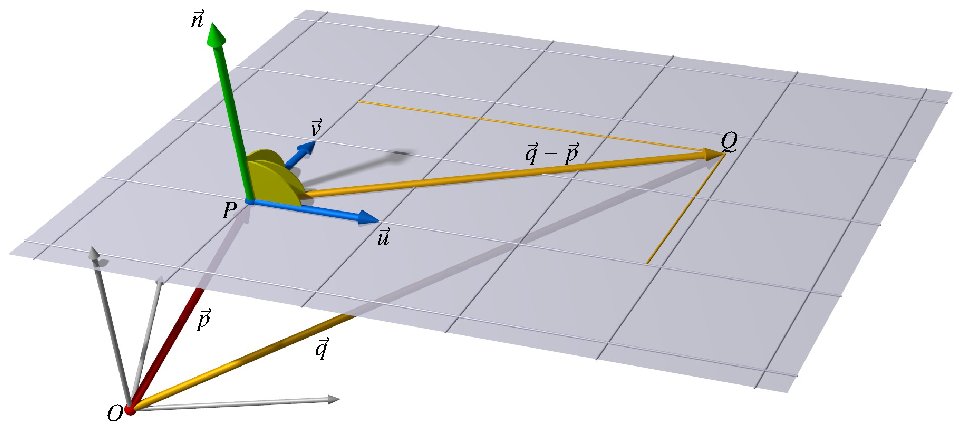
\includegraphics{4/images/normalenform.pdf}
\end{center}
\caption{Ebene in Normalenform\label{image-normalenform}}
\end{figure}
Das Skalarprodukt gibt uns eine neue Möglichkeit, Ebenen zu
beschreiben.
Eine Ebene durch den Punkt $P$ senkrecht auf den Vektor
$\vec n$ besteht genau aus jenen Punkten $Q$, für die der Vektor
$\overset{\rightarrow}{PQ}$ auf $\vec n$ senkrecht steht
(Abbildung~\ref{image-normalenform}).
Mit dem Skalarprodukt
ausgedrückt: Die Menge der Ortsvektoren der Punkte einer Ebene durch $P$ mit
\index{Normale}
Normale $\vec n$ ist
\[
\{\vec r\;|\;(\vec r-\vec p)\cdot \vec n=0\}
\]
Multipliziert man die Gleichung aus, erhält man
\begin{align*}
\left(
\begin{pmatrix}x\\y\\z\end{pmatrix}
-\begin{pmatrix}p_1\\p_2\\p_3\end{pmatrix}\right)\cdot
\begin{pmatrix}n_1\\n_2\\n_3\end{pmatrix}&=0
\\
(x-p_1)n_1+(y-p_2)n_2+(z-p_3)n_3&=0
\\
n_1x+n_2y+n_3z&=p_1n_1+p_2n_2+p_3n_3
\end{align*}
Diese Form der Ebenengleichung, in der $\vec n$ ein Einheitsnormalenvektor ist,
heisst auch {\em Hessesche Normalform}.
\index{Normalenform}
\index{Hessesche Normalform}

\begin{satz}
Ist $\vec n$ ein Einheitsvektor, dann ist
\[
d=(\vec r-\vec p_0)\cdot \vec n
\]
der Abstand des Punktes mit dem Ortsvektor $\vec r$ von der Ebene durch
den Punkt mit Ortsvektor $\vec p_0$ und Normalen $\vec n$.
In Koordinaten:
\[
d=n_xx+n_yy+n_zz-\vec p_0\cdot\vec n
\]
\end{satz}
\begin{proof}[Beweis]
$(\vec r-\vec p)\cdot \vec n$ ist die Länge der Projektion des Vektors
$\vec r -\vec p$ auf den Normalenvektor $\vec n$, also genau der behauptete
Abstand.
\end{proof}

\begin{beispiel}
Man finde die Normalenform der Ebenengleichung (\ref{beispielebene}) auf
Seite~\pageref{beispielebene},
und berechne den Abstand des Punktes $(1,1,1)$ von der Ebene.

\medskip

{\parindent 0pt Die} Lösung vollzieht sich in folgenden Schritten:
\begin{compactenum}
\item Bestimme die Normale der Ebene.
\item Schreibe die Gleichung der Ebene in Normalenform.
\item Bringe die Normalenform in Hessesche Normalform.
\item Berechne den Abstand des Punktes $(1,1,1)$.
\end{compactenum}
Gesucht ist ein Vektor $\vec n$, der auf beiden
Richtungsvektoren senkrecht steht, also
\begin{equation}
\begin{pmatrix}n_1\\n_2\\n_3\end{pmatrix}
\cdot
\begin{pmatrix}2\\2\\-2\end{pmatrix}
=0,
\qquad
\begin{pmatrix}n_1\\n_2\\n_3\end{pmatrix}
\cdot
\begin{pmatrix}3\\-3\\-1\end{pmatrix}
=0
\label{gleichungen-fuer-normale}
\end{equation}
Dies ist gleichbedeutend mit dem Gleichungssystem
\[
\begin{pmatrix}
2&2&-2\\
3&-3&-1
\end{pmatrix}
\begin{pmatrix}n_1\\n_2\\n_3\end{pmatrix}
=\begin{pmatrix}0\\0 \end{pmatrix}
\]
Der Gauss-Algorithmus liefert
\begin{align*}
\begin{tabular}{|>{$}c<{$}>{$}c<{$}>{$}c<{$}|}
\hline
2%
\begin{picture}(0,0)
\color{red}\put(-3,4){\circle{12}}
\end{picture}%
&2&-2\\
3%
\begin{picture}(0,0)%
\color{blue}\drawline(-8,-2)(-8,10)(2,10)(2,-2)
\end{picture}%
&-3&-1\\
\hline
\end{tabular}
&\rightarrow
\begin{tabular}{|>{$}c<{$}>{$}c<{$}>{$}c<{$}|}
\hline
1&1&-1\\
0&-6%
\begin{picture}(0,0)%
\color{red}\put(-7,4){\circle{15}}
\end{picture}%
&2\\
\hline
\end{tabular}
\rightarrow
\begin{tabular}{|>{$}c<{$}>{$}c<{$}>{$}c<{$}|}
\hline
1&1%
\begin{picture}(0,0)
\color{blue}\drawline(-8,10)(-8,-2)(2,-2)(2,10)
\end{picture}%
&-1\\
0&1&-\frac13\\
\hline
\end{tabular}
\rightarrow
\begin{tabular}{|>{$}c<{$}>{$}c<{$}>{$}c<{$}|}
\hline
1&0&-\frac23\\
0&1&-\frac13\\
\hline
\end{tabular}
\end{align*}
Die Komponente $n_3$ ist frei wählbar, wir setzen $n_3=3$, und bekommen
$n_1=2$ und $n_2=1$.
Tatsächlich ist
\begin{align*}
\begin{pmatrix}2\\1\\3\end{pmatrix}
\cdot
\begin{pmatrix}2\\2\\-2\end{pmatrix}
&=4+2-6=0
&
\begin{pmatrix}2\\1\\3\end{pmatrix}
\cdot
\begin{pmatrix}3\\-3\\-1\end{pmatrix}
&=6-3-3=0.
\end{align*}
Damit ist die Normalenform der Ebenengleichung
\begin{align}
\begin{pmatrix}2\\1\\3\end{pmatrix}\cdot\left(
\begin{pmatrix}x\\y\\z\end{pmatrix} - \begin{pmatrix}1\\2\\1\end{pmatrix}
\right)&=0\notag\\
\Rightarrow\qquad
2x+y+3z&=7\label{normalenform}
\end{align}
Diese Form ist zwar eine Normalenform, aber noch nicht die Hessesche
Normalform, da man für diesen Zweck einen Einheitsvektor als
Normalenvektor verwenden muss.
Unser Normalenvektor hat aber die Länge $|\vec n|=\sqrt{14}$.
Dividieren wir die Gleichung (\ref{normalenform})
durch $\sqrt{14}$, erhalten wir die Hessesche Normalform:
\begin{equation}
d=\frac{2}{\sqrt{14}}x+\frac{1}{\sqrt{14}}y+\frac{3}{\sqrt{14}}z-\frac{7}{\sqrt{14}}.
\label{hnf}
\end{equation}
Die Hessesche Normalform berechnet den Abstand eines Punktes von der
Ebene.
Man muss jetzt also nur noch den Punkt $(1,1,1)$ in die  Gleichung
(\ref{hnf}) einsetzen:
\[
d = (2+1+3-7)/\sqrt{14}=-1/\sqrt{14}=-0.26726,
\]
der gesuchte Abstand ist also $d=0.26726$.
\end{beispiel}

%
% Spiegelungen an einer Geraden oder Ebenen
%
\subsection{Spiegelung an einer Geraden oder Ebenen\label{spiegelung}}
\begin{figure}
\begin{center}
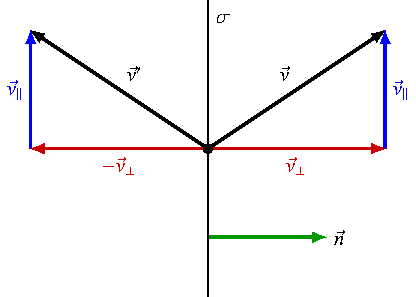
\includegraphics{4/images/spiegelung.pdf}
\end{center}
\caption{Spiegelung eines Vektors $\vec v$ an der Ebene senkrecht auf $\vec n$.
\label{image-spiegelung}}
\end{figure}
Da man mit dem Skalarprodukt senkrechte Projektionen berechnen kann,
muss es auch möglich sein, die Spiegelung eines Vektors $\vec v$
an einer Ebene mit Normale $\vec n$ zu berechnen ($|\vec n|=1$).
Dazu zerlegt man den Vektor $\vec v$ in eine Komponente $\vec v_{\|}$
parallel zur Ebene und eine Komponenten $\vec v_{\perp}$ senkrecht dazu,
also $\vec v=\vec v_{\|}+\vec v_{\perp}$ (Abbildung~\ref{image-spiegelung}).
Die senkrechte Komponente
ist im wesentlichen die Projektion von $\vec v$ auf $\vec n$:
\[
\vec v_{\perp}=
(\vec v\cdot\vec n)\vec n
.
\]
Die parallele Komponente ist der Rest:
\[
\vec v_{\|}=\vec v -\vec v_{\perp}=
\vec v-(\vec v\cdot\vec n)\vec n
,
\]
Beim gespiegelten Vektor zeigt die senkrechte Komponente in die
entgegengesetzte Richtung:
\begin{equation}
\vec v_{\text{gespiegelt}}=
\vec v_{\|}-\vec v_{\perp}
=
\vec v-(\vec v\cdot\vec n)\vec n
-
(\vec v\cdot\vec n)\vec n
=\vec v-2(\vec v\cdot\vec n)\vec n.
\label{equation:spiegelung}
\end{equation}

\begin{beispiel}
Man spiegle den Vektor $\vec a$ an der Ebene mit der Normalen $\vec n$,
\[
\vec a=\begin{pmatrix}1\\2\\3\end{pmatrix},
\qquad
\vec n=\begin{pmatrix}1\\1\\1\end{pmatrix}
\]

\smallskip

{\parindent 0pt Zunächst stellen wir fest,} dass $\vec n$ noch
kein Einheitsvektor ist, dass wir stattdessen $\vec n_0=\vec n/\sqrt{3}$
verwenden müssen.
Damit kann $\vec a$ jetzt die parallelen und orthogonalen
Komponenten zerlegt werden:
\[
\vec a_{\perp}=(\vec a\cdot\vec n_0)\vec n_0
=\frac1{\sqrt{3}} (1+2+3)\frac1{\sqrt{3}}\begin{pmatrix}1\\1\\1\end{pmatrix}
=\begin{pmatrix}2\\2\\2\end{pmatrix},
\quad
\vec a_{\|}=\begin{pmatrix} -1\\0\\1 \end{pmatrix}.
\]
Nach Formel (\ref{equation:spiegelung}) ist
\[
\vec a'=\vec a_{\|}-\vec a_{\perp}
=
\begin{pmatrix}-1\\0\\1\end{pmatrix}-\begin{pmatrix}2\\2\\2\end{pmatrix}
=\begin{pmatrix}-3\\-2\\-1\end{pmatrix}.
\]
der gespiegelt Vektor.
\end{beispiel}



